\documentclass{standalone}
\usepackage{tikz}
\usetikzlibrary{patterns, positioning}
\usepackage[sfdefault]{ClearSans} %% option 'sfdefault' activates Clear Sans as the default text font
\usepackage[T1]{fontenc}

\begin{document}
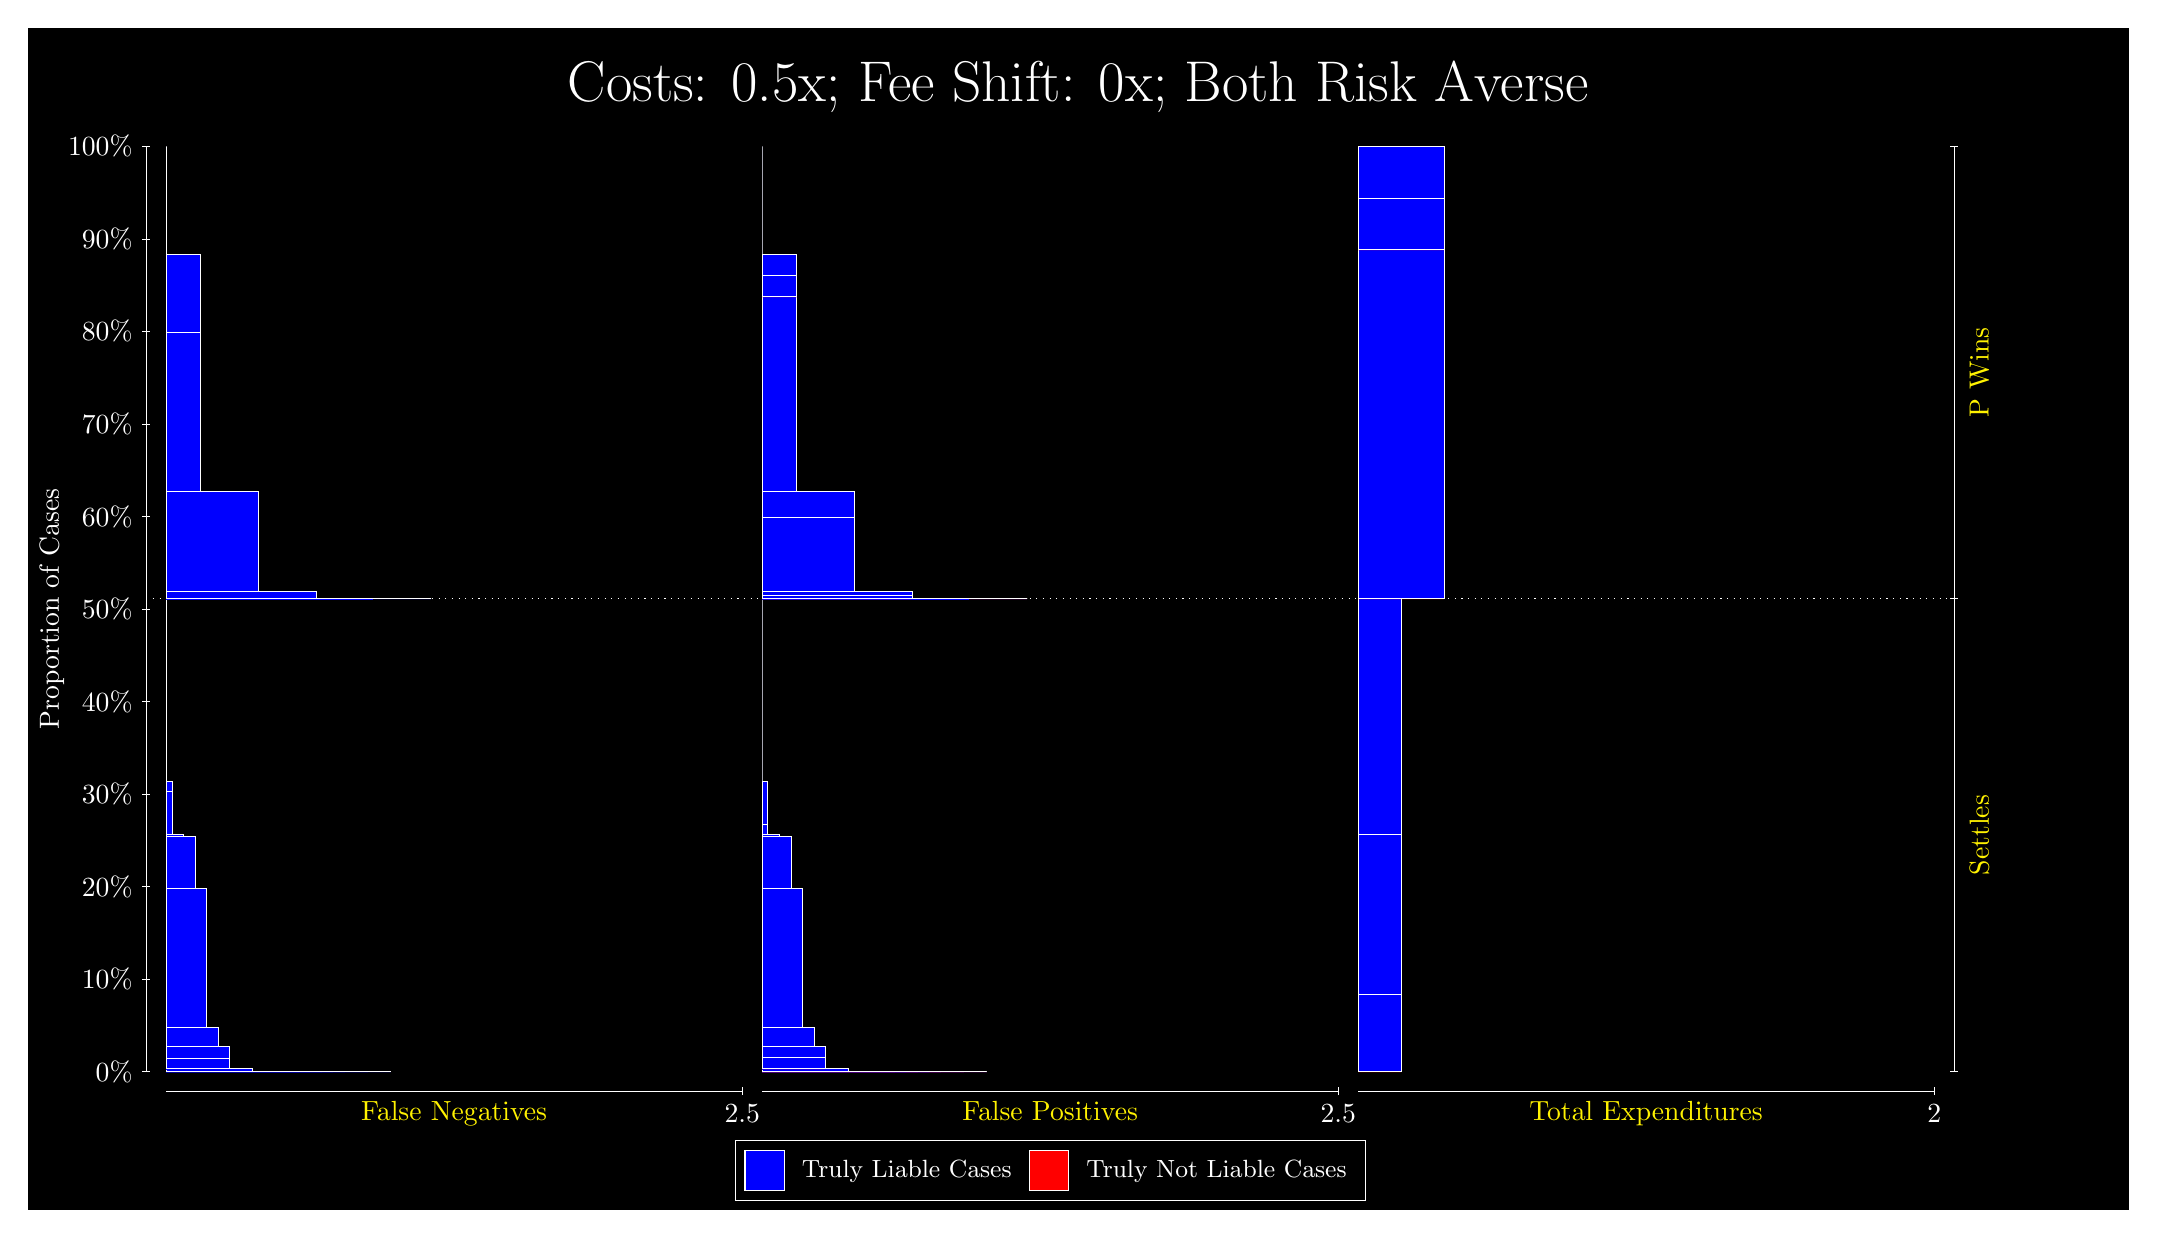
\begin{tikzpicture}
\draw[fill=black] (0,0) rectangle (26.667,15);
\draw[text=white] (0,13.5) rectangle (26.667,15) node[midway] {\huge Costs: 0.5x; Fee Shift: 0x; Both Risk Averse};
\draw[white, very thin] (1.5,1.75) -- (1.5,13.5);
\node[rotate=90, text=white, anchor=center] at (0.3, 7.625) {Proportion of Cases};
\draw[white, very thin] (1.45,1.75) -- (1.55,1.75);
\node[text=white, anchor=east] at (1.45, 1.75) {0\%};
\draw[white, very thin] (1.45,2.925) -- (1.55,2.925);
\node[text=white, anchor=east] at (1.45, 2.925) {10\%};
\draw[white, very thin] (1.45,4.1) -- (1.55,4.1);
\node[text=white, anchor=east] at (1.45, 4.1) {20\%};
\draw[white, very thin] (1.45,5.275) -- (1.55,5.275);
\node[text=white, anchor=east] at (1.45, 5.275) {30\%};
\draw[white, very thin] (1.45,6.45) -- (1.55,6.45);
\node[text=white, anchor=east] at (1.45, 6.45) {40\%};
\draw[white, very thin] (1.45,7.625) -- (1.55,7.625);
\node[text=white, anchor=east] at (1.45, 7.625) {50\%};
\draw[white, very thin] (1.45,8.8) -- (1.55,8.8);
\node[text=white, anchor=east] at (1.45, 8.8) {60\%};
\draw[white, very thin] (1.45,9.975) -- (1.55,9.975);
\node[text=white, anchor=east] at (1.45, 9.975) {70\%};
\draw[white, very thin] (1.45,11.15) -- (1.55,11.15);
\node[text=white, anchor=east] at (1.45, 11.15) {80\%};
\draw[white, very thin] (1.45,12.325) -- (1.55,12.325);
\node[text=white, anchor=east] at (1.45, 12.325) {90\%};
\draw[white, very thin] (1.45,13.5) -- (1.55,13.5);
\node[text=white, anchor=east] at (1.45, 13.5) {100\%};

\draw[white, very thin] (24.457,1.75) -- (24.457,13.5);
\draw[white, very thin] (24.407,1.75) -- (24.507,1.75);
\node[anchor=west] at (24.407, 1.75) {};
\draw[white, very thin] (24.407,7.7565) -- (24.507,7.7565);
\node[anchor=west] at (24.407, 7.7565) {};
\draw[white, very thin] (24.407,13.5) -- (24.507,13.5);
\node[anchor=west] at (24.407, 13.5) {};

\draw[white, very thin, fill=blue] (1.75,1.75) rectangle (4.6044,1.75);
\draw[white, very thin, fill=blue] (1.75,1.75) rectangle (4.3116,1.75);
\draw[white, very thin, fill=blue] (1.75,1.75) rectangle (4.0188,1.75);
\draw[white, very thin, fill=blue] (1.75,1.75) rectangle (3.8725,1.75);
\draw[white, very thin, fill=blue] (1.75,1.75) rectangle (3.7261,1.75);
\draw[white, very thin, fill=blue] (1.75,1.75) rectangle (3.5797,1.75);
\draw[white, very thin, fill=blue] (1.75,1.75) rectangle (3.4333,1.75);
\draw[white, very thin, fill=blue] (1.75,1.75) rectangle (3.287,1.7506);
\draw[white, very thin, fill=blue] (1.75,1.7506) rectangle (3.1406,1.7523);
\draw[white, very thin, fill=blue] (1.75,1.7523) rectangle (2.9942,1.7523);
\draw[white, very thin, fill=blue] (1.75,1.7523) rectangle (2.8478,1.7866);
\draw[white, very thin, fill=blue] (1.75,1.7866) rectangle (2.7015,1.7875);
\draw[white, very thin, fill=blue] (1.75,1.7875) rectangle (2.5551,1.9235);
\draw[white, very thin, fill=blue] (1.75,1.9235) rectangle (2.5551,2.0673);
\draw[white, very thin, fill=blue] (1.75,2.0673) rectangle (2.4087,2.3127);
\draw[white, very thin, fill=blue] (1.75,2.3127) rectangle (2.2623,2.3129);
\draw[white, very thin, fill=blue] (1.75,2.3129) rectangle (2.2623,4.0759);
\draw[white, very thin, fill=blue] (1.75,4.0759) rectangle (2.1159,4.7416);
\draw[white, very thin, fill=blue] (1.75,4.7416) rectangle (1.9696,4.7648);
\draw[white, very thin, fill=blue] (1.75,4.7648) rectangle (1.8232,5.3059);
\draw[white, very thin, fill=blue] (1.75,5.3059) rectangle (1.8232,5.4305);
\draw[white, very thin, fill=red] (1.75,5.4305) rectangle (1.75,5.4305);
\draw[white, very thin, fill=blue] (1.75,5.4305) rectangle (1.75,7.7565);
\draw[white, very thin, fill=blue] (1.75,7.7565) rectangle (5.1167,7.7565);
\draw[white, very thin, fill=blue] (1.75,7.7565) rectangle (4.3848,7.7574);
\draw[white, very thin, fill=blue] (1.75,7.7574) rectangle (3.6529,7.8482);
\draw[white, very thin, fill=blue] (1.75,7.8482) rectangle (2.921,9.1211);
\draw[white, very thin, fill=blue] (1.75,9.1211) rectangle (2.1891,11.136);
\draw[white, very thin, fill=blue] (1.75,11.136) rectangle (2.1891,12.135);
\draw[white, very thin, fill=red] (1.75,12.135) rectangle (1.75,12.135);
\draw[white, very thin, fill=blue] (1.75,12.135) rectangle (1.75,13.5);
\draw[white, very thin, fill=red] (9.3189,1.75) rectangle (12.173,1.75);
\draw[white, very thin, fill=blue] (9.3189,1.75) rectangle (12.173,1.75);
\draw[white, very thin, fill=red] (9.3189,1.75) rectangle (11.88,1.75);
\draw[white, very thin, fill=blue] (9.3189,1.75) rectangle (11.88,1.75);
\draw[white, very thin, fill=red] (9.3189,1.75) rectangle (11.588,1.75);
\draw[white, very thin, fill=blue] (9.3189,1.75) rectangle (11.588,1.75);
\draw[white, very thin, fill=blue] (9.3189,1.75) rectangle (11.441,1.75);
\draw[white, very thin, fill=red] (9.3189,1.75) rectangle (11.295,1.75);
\draw[white, very thin, fill=blue] (9.3189,1.75) rectangle (11.295,1.75);
\draw[white, very thin, fill=blue] (9.3189,1.75) rectangle (11.149,1.75);
\draw[white, very thin, fill=red] (9.3189,1.75) rectangle (11.002,1.75);
\draw[white, very thin, fill=blue] (9.3189,1.75) rectangle (11.002,1.75);
\draw[white, very thin, fill=blue] (9.3189,1.75) rectangle (10.856,1.7506);
\draw[white, very thin, fill=red] (9.3189,1.7506) rectangle (10.709,1.7506);
\draw[white, very thin, fill=blue] (9.3189,1.7506) rectangle (10.709,1.7523);
\draw[white, very thin, fill=blue] (9.3189,1.7523) rectangle (10.563,1.7523);
\draw[white, very thin, fill=red] (9.3189,1.7523) rectangle (10.417,1.7523);
\draw[white, very thin, fill=blue] (9.3189,1.7523) rectangle (10.417,1.7866);
\draw[white, very thin, fill=blue] (9.3189,1.7866) rectangle (10.27,1.7875);
\draw[white, very thin, fill=red] (9.3189,1.7875) rectangle (10.124,1.7875);
\draw[white, very thin, fill=blue] (9.3189,1.7875) rectangle (10.124,1.9313);
\draw[white, very thin, fill=blue] (9.3189,1.9313) rectangle (10.124,2.0673);
\draw[white, very thin, fill=blue] (9.3189,2.0673) rectangle (9.9776,2.3127);
\draw[white, very thin, fill=red] (9.3189,2.3127) rectangle (9.8312,2.3127);
\draw[white, very thin, fill=blue] (9.3189,2.3127) rectangle (9.8312,4.0757);
\draw[white, very thin, fill=blue] (9.3189,4.0757) rectangle (9.8312,4.0759);
\draw[white, very thin, fill=blue] (9.3189,4.0759) rectangle (9.6848,4.7416);
\draw[white, very thin, fill=blue] (9.3189,4.7416) rectangle (9.5384,4.7649);
\draw[white, very thin, fill=blue] (9.3189,4.7649) rectangle (9.3921,4.8896);
\draw[white, very thin, fill=blue] (9.3189,4.8896) rectangle (9.3921,5.4306);
\draw[white, very thin, fill=blue] (9.3189,5.4306) rectangle (9.3189,7.7565);
\draw[white, very thin, fill=red] (9.3189,7.7565) rectangle (12.686,7.7565);
\draw[white, very thin, fill=blue] (9.3189,7.7565) rectangle (12.686,7.7565);
\draw[white, very thin, fill=red] (9.3189,7.7565) rectangle (11.954,7.7565);
\draw[white, very thin, fill=blue] (9.3189,7.7565) rectangle (11.954,7.7567);
\draw[white, very thin, fill=blue] (9.3189,7.7567) rectangle (11.954,7.7574);
\draw[white, very thin, fill=red] (9.3189,7.7574) rectangle (11.222,7.7574);
\draw[white, very thin, fill=blue] (9.3189,7.7574) rectangle (11.222,7.8024);
\draw[white, very thin, fill=blue] (9.3189,7.8024) rectangle (11.222,7.8482);
\draw[white, very thin, fill=red] (9.3189,7.8482) rectangle (10.49,7.8482);
\draw[white, very thin, fill=blue] (9.3189,7.8482) rectangle (10.49,8.7832);
\draw[white, very thin, fill=blue] (9.3189,8.7832) rectangle (10.49,9.1211);
\draw[white, very thin, fill=blue] (9.3189,9.1211) rectangle (9.758,11.592);
\draw[white, very thin, fill=red] (9.3189,11.592) rectangle (9.758,11.592);
\draw[white, very thin, fill=blue] (9.3189,11.592) rectangle (9.758,11.864);
\draw[white, very thin, fill=blue] (9.3189,11.864) rectangle (9.758,12.135);
\draw[white, very thin, fill=blue] (9.3189,12.135) rectangle (9.3189,13.5);
\draw[white, very thin, fill=red] (16.888,1.75) rectangle (17.437,1.75);
\draw[white, very thin, fill=blue] (16.888,1.75) rectangle (17.437,2.7308);
\draw[white, very thin, fill=red] (16.888,2.7308) rectangle (17.437,2.7308);
\draw[white, very thin, fill=blue] (16.888,2.7308) rectangle (17.437,4.7658);
\draw[white, very thin, fill=red] (16.888,4.7658) rectangle (17.437,4.7658);
\draw[white, very thin, fill=blue] (16.888,4.7658) rectangle (17.437,7.7565);
\draw[white, very thin, fill=red] (16.888,7.7565) rectangle (17.986,7.7565);
\draw[white, very thin, fill=blue] (16.888,7.7565) rectangle (17.986,12.188);
\draw[white, very thin, fill=red] (16.888,12.188) rectangle (17.986,12.188);
\draw[white, very thin, fill=blue] (16.888,12.188) rectangle (17.986,12.844);
\draw[white, very thin, fill=red] (16.888,12.844) rectangle (17.986,12.844);
\draw[white, very thin, fill=blue] (16.888,12.844) rectangle (17.986,13.5);
\draw[white, dotted] (1.5,7.7565) -- (24.457,7.7565);
\draw[white, very thin] (1.75,1.5) -- (9.0689,1.5);
\node[text=yellow, anchor=north] at (5.4094, 1.5) {False Negatives};
\draw[white, very thin] (9.0689,1.45) -- (9.0689,1.55);
\node[text=white, anchor=north] at (9.0689, 1.45) {2.5};

\draw[white, very thin] (9.3189,1.5) -- (16.638,1.5);
\node[text=yellow, anchor=north] at (12.978, 1.5) {False Positives};
\draw[white, very thin] (16.638,1.45) -- (16.638,1.55);
\node[text=white, anchor=north] at (16.638, 1.45) {2.5};

\draw[white, very thin] (16.888,1.5) -- (24.207,1.5);
\node[text=yellow, anchor=north] at (20.547, 1.5) {Total Expenditures};
\draw[white, very thin] (24.207,1.45) -- (24.207,1.55);
\node[text=white, anchor=north] at (24.207, 1.45) {2};

\node[text=yellow, centered, rotate=90] at (24.777, 4.7532) {Settles};
\node[text=yellow, centered, rotate=90] at (24.777, 10.628) {P Wins};

\draw (12.978300999999998,1.5) node[draw=none] (baseCoordinate) {};
\begin{scope}[align=center]
        \matrix[scale=0.5, draw=white, below=0.5cm of baseCoordinate, nodes={draw}, column sep=0.1cm]{
            \node[rectangle, draw, minimum width=0.5cm, minimum height=0.5cm, fill=blue] {}; &
            \node[draw=none, font=\small, text=white] (B) {Truly Liable Cases}; &
            \node[rectangle, draw, minimum width=0.5cm, minimum height=0.5cm, fill=red] {}; &
            \node[draw=none, font=\small, text=white] (B) {Truly Not Liable Cases}; \\
            };
\end{scope}

\end{tikzpicture}
\end{document}